% Section content template for individual Educative lessons
% This file contains the actual content for a specific section
% Generated from Educative API section content

% Section: Key Concepts to Prepare for the System Design Interview
% Section ID: 4705505809661952
% Section Slug: key-concepts-to-prepare-for-the-system-design-interview
% Generated: 2025-08-02T19:56:18.910890

In a System Design Interview, interviewers ask the candidate to design a web-scale application. For example, they might ask to design platforms like \href{https://www.educative.io/courses/grokking-the-system-design-interview/system-design-instagram}{\ul{Instagram}}, \href{https://www.educative.io/courses/grokking-the-system-design-interview/system-design-youtube}{YouTube}, or \href{https://www.educative.io/courses/grokking-the-system-design-interview/system-design-uber}{\ul{Uber backend}}.

Unlike a coding interview question, System Design Interviews are free-form discussions with no right or wrong answer. Instead , the interviewer is trying to evaluate the candidate's ability to discuss the different aspects of the system and assess the solution based on the requirements that might evolve during the conversation.

The best way to imagine the conversation is that we and our colleagues are asked to design a large-scale system. We have hashed out the details on the whiteboard, and we understand the requirements, scope, and constraints before proposing a solution.

So, how do we design a system in an interview if we have never built one in real life? To crack the System Design interview, we'll need to prepare in four areas:

\begin{enumerate}
\item
\phantomsection\label{sytf57PllWobmyQmw6daA}
Fundamental concepts in System Design interview
\item
\phantomsection\label{C9bbfB2bmR6Q8zH_uli46}
Fundamentals of distributed system
\item
\phantomsection\label{nIOMkubVDfxaL-82Zl6a-}
The architecture of large-scale web applications
\item
\phantomsection\label{fZTijF1c8rfdHYH2hGOLh}
Design of large-scale distributed systems
\end{enumerate}

Each of these dimensions flows into the next.

\subsection{Why is it important to prepare strategically?}\label{c7fQXsCm-3QaDyPNyBa8p}

How we prepare for an interview at Amazon will probably differ from how we'd prepare for one at Slack. While the overall interview process shares similarities across various companies, there are also distinct differences that we must prepare for. This is one of the reasons why preparing strategically is so important. We 'll feel more confident in the long run if we're intentional and thorough when creating an interview prep plan.

If we don't know the fundamentals, we won't be prepared to architect a service; if we don't know how to put those systems together, we won't be able to design a specific solution; once we've designed large-scale systems, we can apply the lessons learned to enhance our base knowledge.

Let's look at each of these dimensions.

\begin{quote}
\textbf{Preparing for the System Design interview}

\subsection{System Design interview}

\subsubsection{Fundamental concepts in System Design interview}

\begin{itemize}
\item PACELC theorem
\item Heartbeat
\item AJAX polling/HTTP short-polling
\item HTTP long-polling
\item WebSockets
\item Server-sent events (SSEs)
\end{itemize}
\subsubsection{Fundamentals of distributed system}

\begin{itemize}
\item Durability
\item Replication
\item Partitioning
\item Consensus
\end{itemize}
\subsubsection{The architecture of large-scale web applications}

\begin{itemize}
\item HTTP \& REST
\item Caching
\item CDNs
\item N-Tier applications
\end{itemize}
\subsubsection{Design of large-scale distributed systems}

\end{quote}

\subsection{Fundamental concepts in System Design interview}\label{6AuT2aNjnlxXD_1OxAsQN}

In this lesson, we'll explore some concepts that are important for the System Design interview.

\subsubsection{PACELC theorem}\label{fmWp0a_r8F2Lmz_1Z5SxJ}

The CAP theorem doesn't answer the question: ``What choices does a distributed system have when there are no network partitions?''. The PACELC theorem answers this question.

The PACELC theorem states the following about a system that replicates data:

\begin{itemize}
\item
\phantomsection\label{oiv9GjYixGLMIND24PUeH}
if\ statement: A distributed system can tradeoff between availability and consistency if there's a partition.
\item
\phantomsection\label{dWs-lwrWIqBLFxlX6tEZj}
else\ statement: When the system normally runs without partitions, the system can tradeoff between latency and consistency.
\end{itemize}

\begin{figure}[htbp]
 \centering
 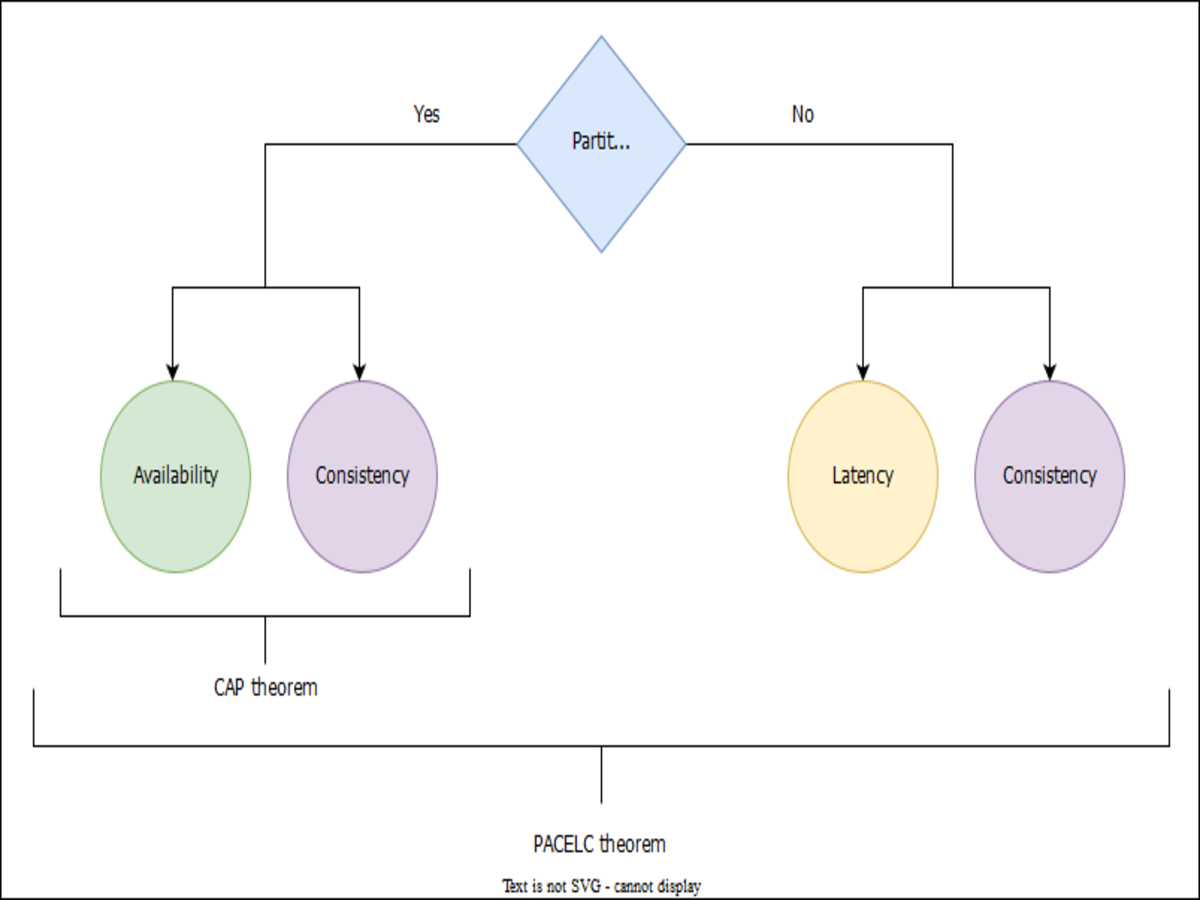
\includegraphics[width=0.8\textwidth]{Images/chapter_1/section_4705505809661952/5540989725179904.png}
 \caption{The flow of the PACELC theorem}
\end{figure}

The first three letters of the theorem, PAC, are the same as the CAP theorem. The ELC is the extension here. The theorem assumes we maintain high availability by replication. When there's a failure, the CAP theorem prevails. If there isn't a failure, we still have to consider the tradeoff between consistency and latency of a replicated system.

Examples of a PC/EC system include BigTable and HBase. They 'll always choose consistency, giving up availability and lower latency. Examples of a PA/EL system include Dynamo and Cassandra. They choose availability over consistency when a partition occurs. Otherwise
, they choose lower latency. An example of a PA/EC system is MongoDB. In the case of a partition, it chooses availability but otherwise guarantees consistency.

\subsubsection{Heartbeat}\label{jsbU1NcYO3HigIlOhro6_}

A \textbf{heartbeat message} is a mechanism that helps us detect failures in a distributed system. If there's a central server, all servers periodically send a heartbeat message to it to show that it's still alive and functioning. If there's no central server, all servers randomly select a set of servers and send that set a heartbeat message every few seconds. This way, if there are no heartbeat messages received for awhile, the system can suspect there might be a failure or a crash.

\subsubsection{AJAX polling}\label{enUJIr-lZgGNXvH3Wjdd0}

Polling is a standard technique used by most AJAX apps. The idea is that the client repeatedly polls a server for data. The client makes a request and waits for the server to respond with data. If no data is available, the server returns an empty response.

\begin{figure}[htbp]
 \centering
 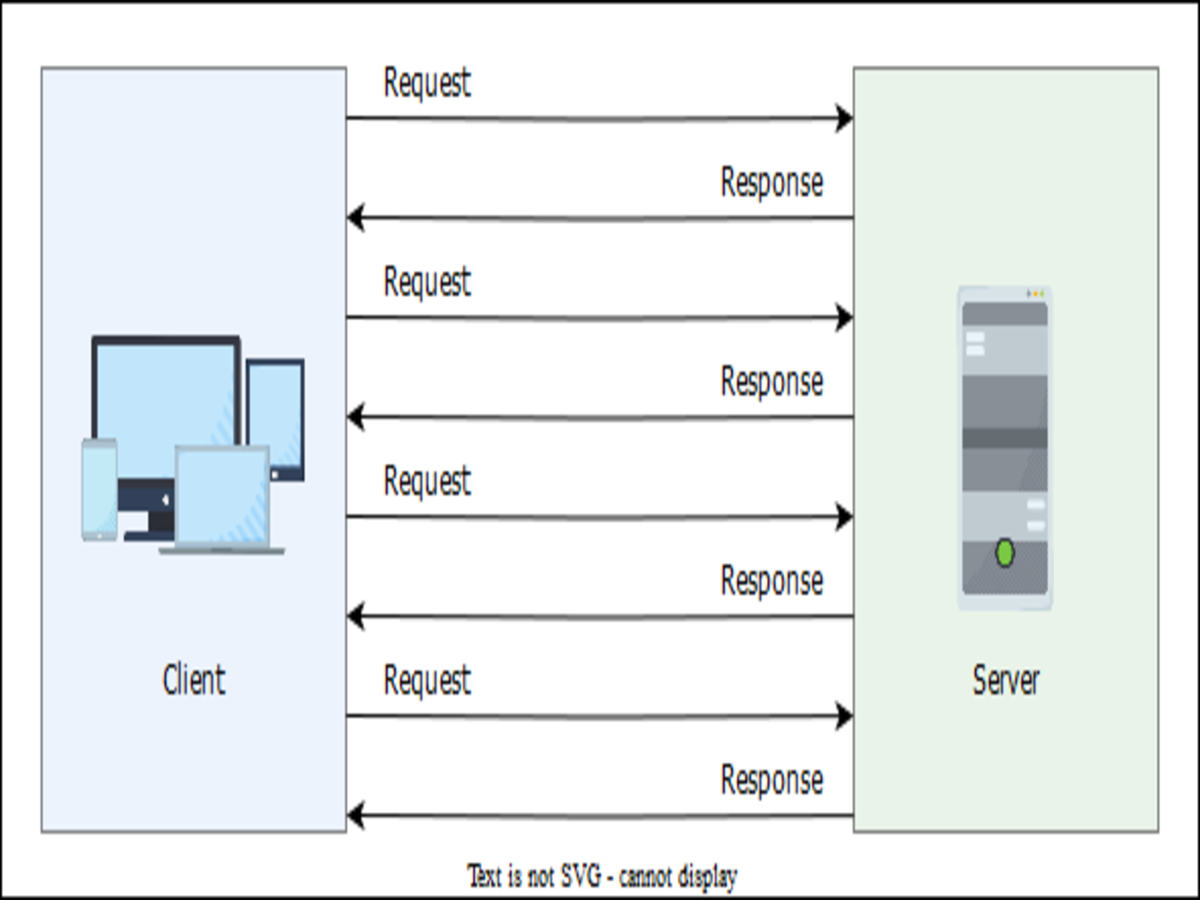
\includegraphics[width=0.8\textwidth]{Images/chapter_1/section_4705505809661952/4686911117852672.png}
 \caption{AJAX polling}
\end{figure}

\subsubsection{HTTP long-polling}\label{5mssFgfSXzfw1y8hNKUGN}

With long-polling, the client requests information from the server, but the server may not respond immediately. This technique is sometimes called \textbf{hanging GET}. If the server doesn't have any available data for the client, it'll hold the request and wait until there is data available instead of sending an empty response. Once the data becomes available, a full response is sent to the client. The client immediately re-requests information from the server so that the server will almost always have an available waiting request that it can use to deliver data in response to an event.

\begin{figure}[htbp]
 \centering
 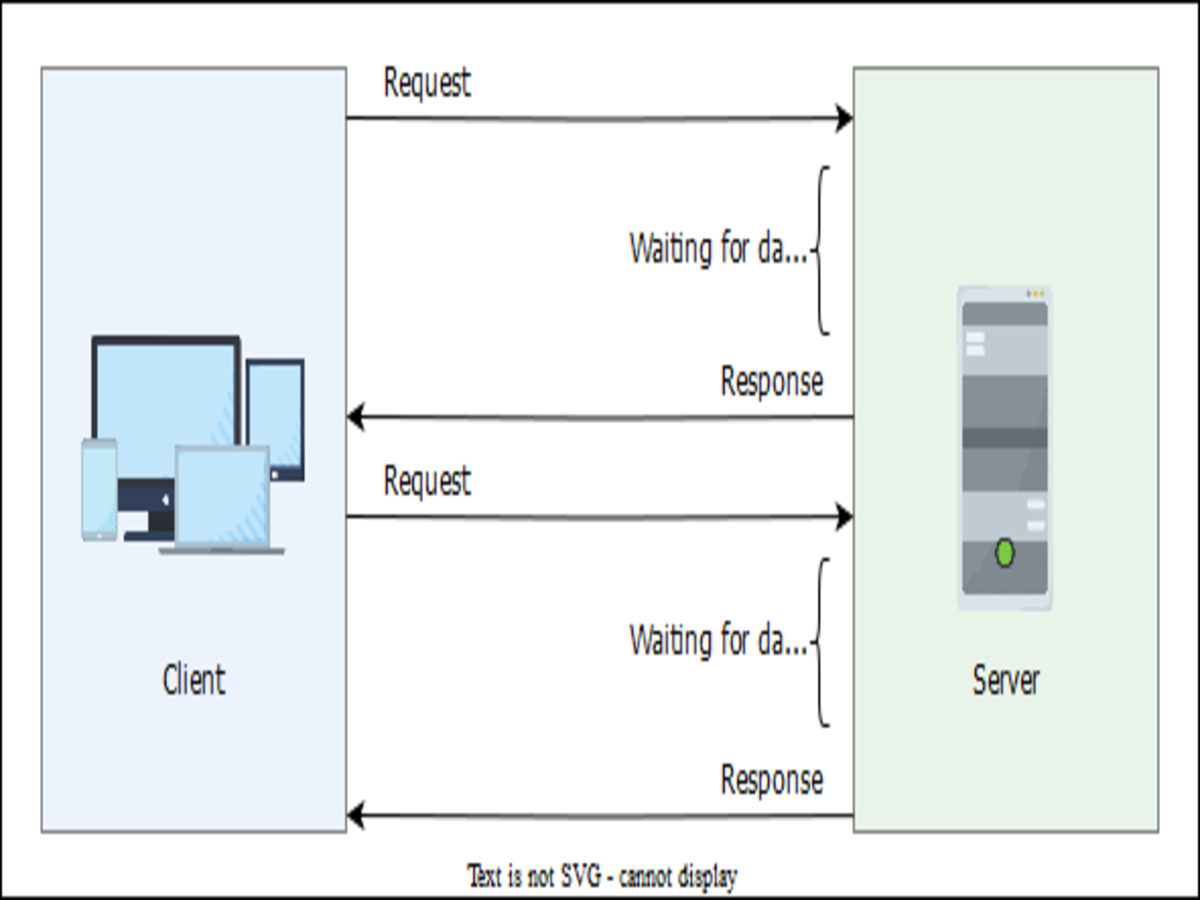
\includegraphics[width=0.8\textwidth]{Images/chapter_1/section_4705505809661952/5275089138745344.png}
 \caption{HTTP long-polling}
\end{figure}

\subsubsection{WebSockets}\label{a6a8mQ97j6bQeKXlTtNmQ}

\textbf{WebSocket} provides full-duplex communication channels over a single TCP connection. It provides a persistent connection between a client and a server. Both parties can use this connection to start sending data at any time. The client establishes a connection through a WebSocket handshake. If the process succeeds, the server and client can begin exchanging data in both directions at any time.

\begin{figure}[htbp]
 \centering
 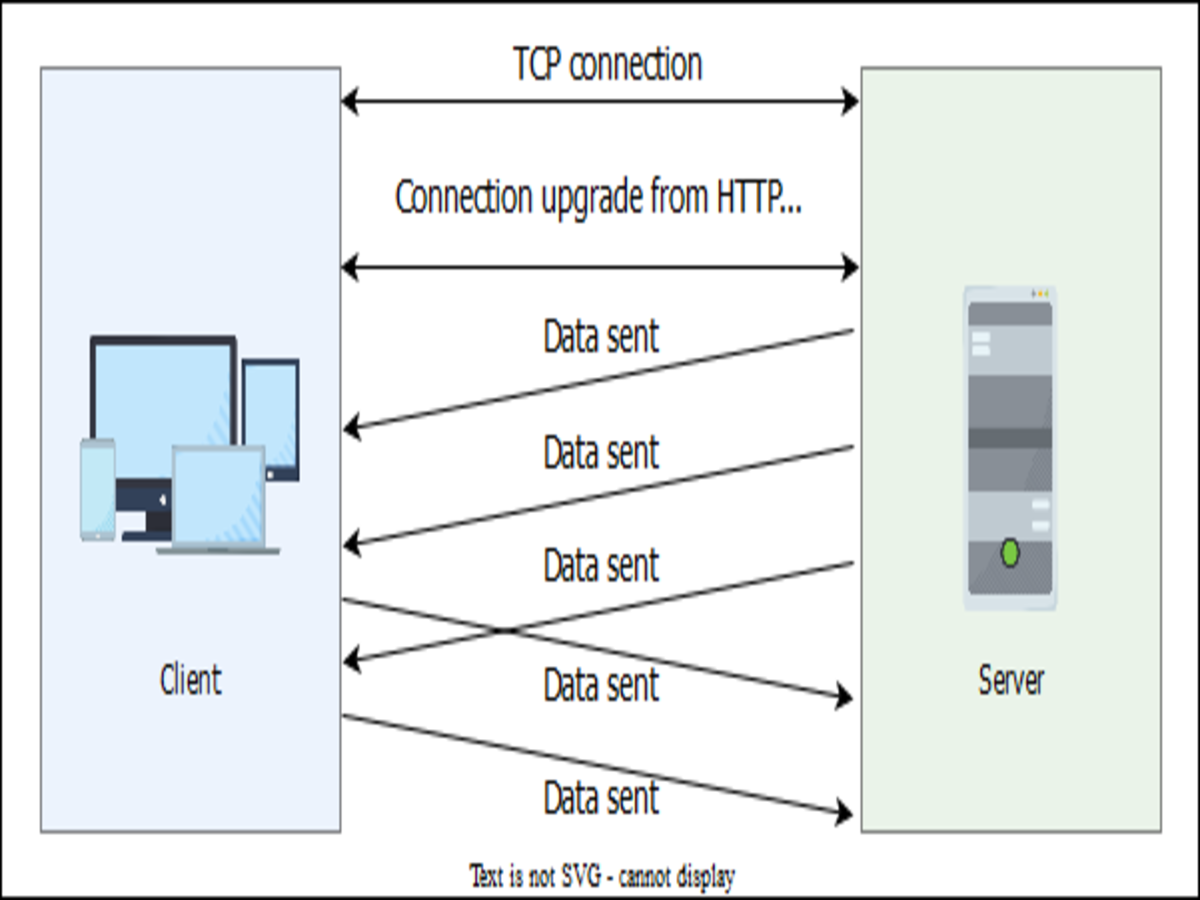
\includegraphics[width=0.8\textwidth]{Images/chapter_1/section_4705505809661952/6099513748357120.png}
 \caption{Full-duplex communication using WebSockets}
\end{figure}

\subsubsection{Server-sent events (SSEs)}\label{clSmpjY3b6-ZaeLvydfLG}

A client can establish a long-term connection with a server using SSEs. The server uses this connection to send data to a client. If the client wants to send data to the server, it would require the use of another technology or protocol.

\begin{figure}[htbp]
 \centering
 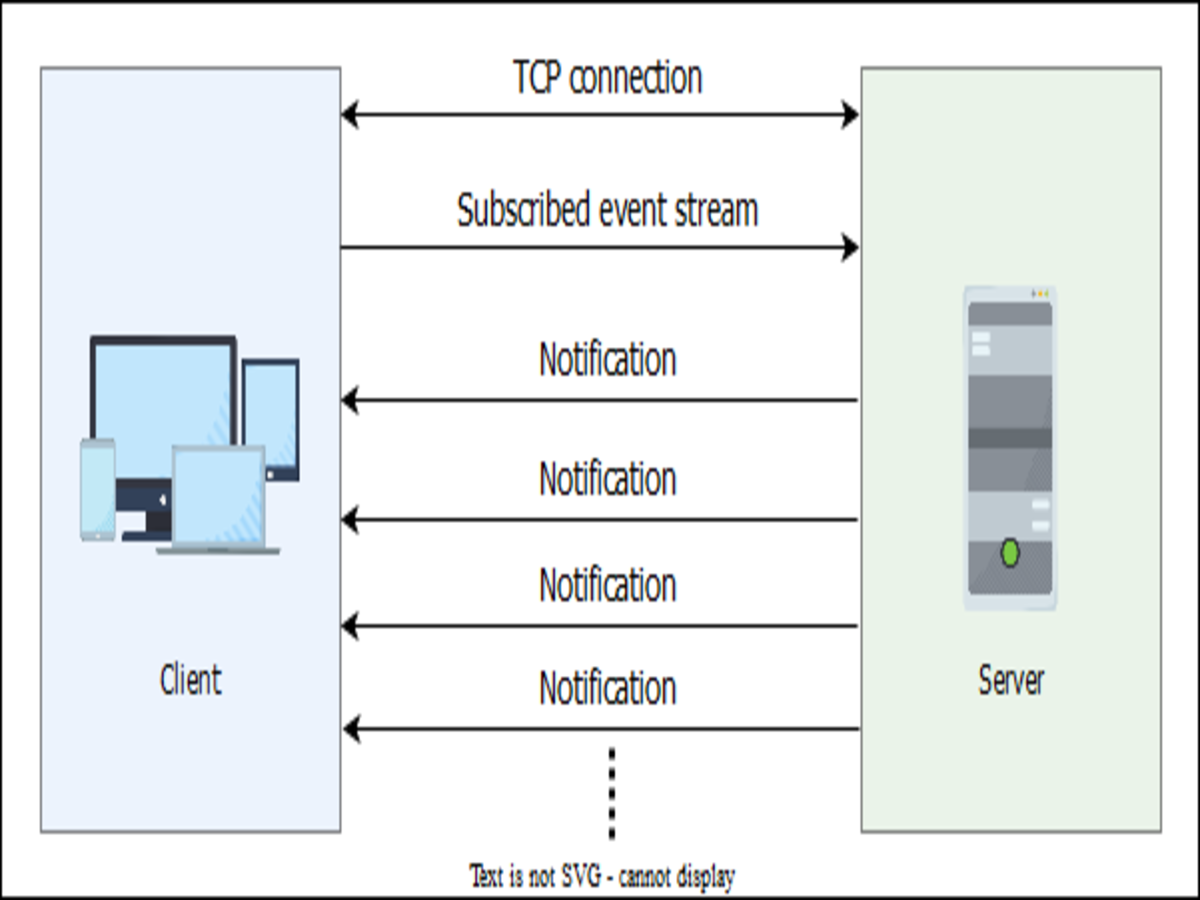
\includegraphics[width=0.8\textwidth]{Images/chapter_1/section_4705505809661952/5728562590384128.png}
 \caption{Server-sent events (SSE)}
\end{figure}

\subsubsection{Fundamentals of distributed system}\label{PKCzJ8uMmQpxBqvnVoddk}

Like with anything else, it is important to start with the basics. The fundamentals of distributed systems can give us the framework of what's possible and what's not in a given system.

We can understand the limitations of specific architectures and the trade-offs needed to achieve particular goals (e.g., consistency vs. write throughput). At the most basic level, we must start with the strengths, weaknesses, and purposes of distributed systems. We need to be able to discuss topics like:

\paragraph{Data durability and consistency}\label{iHwKHOH3Na9dIlJQHakjJ}

We must understand the differences and impacts of storage solution failure and corruption rates in read-write processes.

\paragraph{Replication}\label{zZc2L079kvHI0bXWlCpGQ}

Replication is the key to unlocking data durability and consistency. It deals with backing up data but also with repeating processes at scale.

\paragraph{Partitioning}\label{zghAEVLGuomGBtE2nf5S3}

Also called sharding; partitions divide data across different nodes within our system. As replication distributes data across nodes, partitioning distributes processes across nodes, reducing the reliance on pure replication.

\paragraph{Consensus}\label{dOF9E5f97ZsQ5pfhYB8LW}

One of our nodes is in Seattle, another is in Beijing, and another is in London. There is a system request at 7:05 a.m. Pacific Daylight Time. Given the travel time of data packets, can this be recorded and properly synchronized in the remote nodes, and can it be concurred? This is a simple problem of consensus---all the nodes need to agree, which will prevent faulty processes from running and ensure consistency and replication of data and processes across the system.

\begin{figure}[htbp]
 \centering
 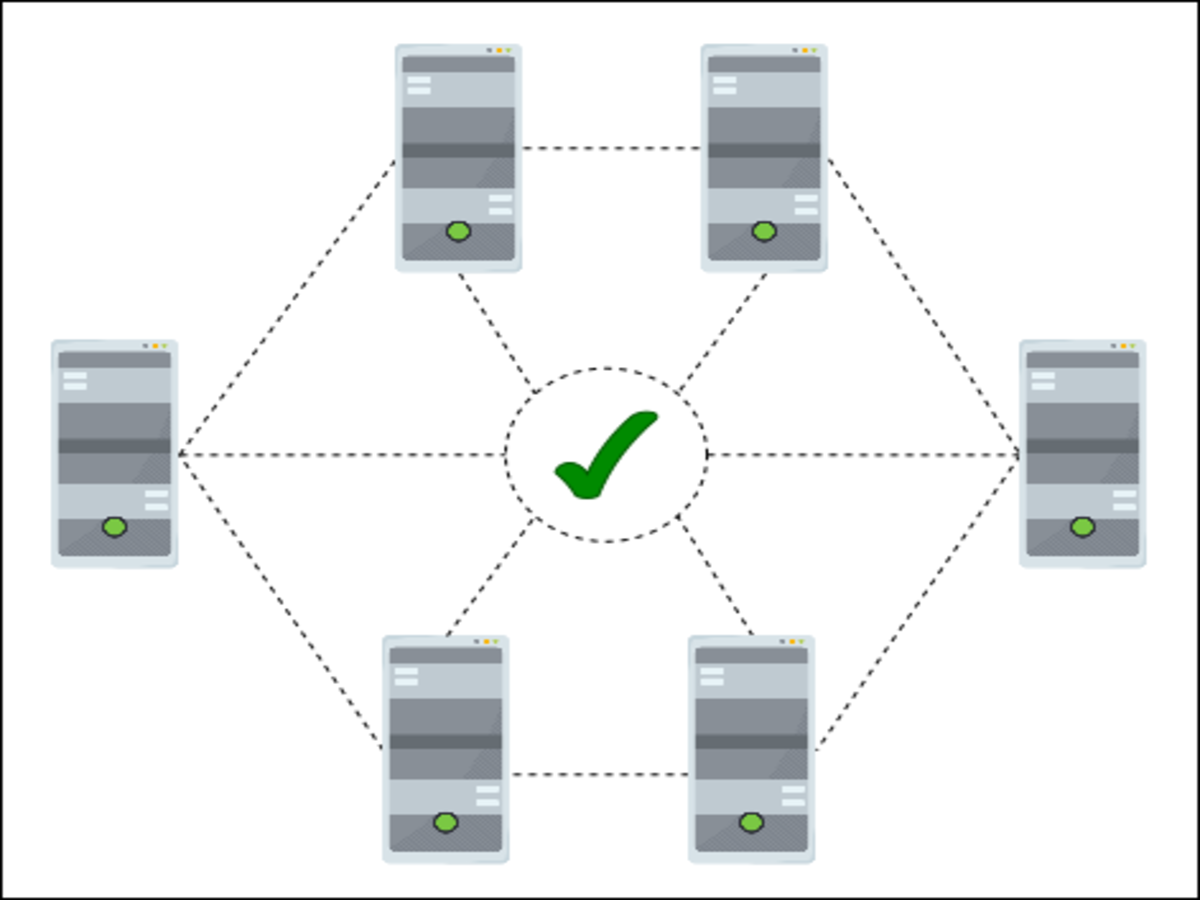
\includegraphics[width=0.8\textwidth]{Images/chapter_1/section_4705505809661952/5038218840244224.png}
 \caption{Consensus in System Design}
\end{figure}

\paragraph{Distributed transactions}\label{A1p1J6i6wVyaN0N9gZ-t3}

Once we've achieved consensus, now transactions from applications need to be committed across databases, with fault checks performed by each involved resource. Two -way and three-way communication to read, write, and commit are shared across participant nodes.

\subsubsection{The architecture of large-scale web applications}\label{3p8svxAoCHpdZLejxHViu}

We already know that most large-scale applications are web applications. Even if it's not, the major consumer platforms like Netflix, Twitter, and Amazon, enterprises are moving away from on-premises systems like Exchange to cloud solutions from Microsoft, Google, and AWS. That 's why it's good to understand the architecture of such systems.

We need to learn about topics such as:

\paragraph{N-tier applications}\label{w2_JW1jZ-X5kbVp55LzMo}

Processing happens at various levels in a distributed system. Some processes are on the client, some on the server, and others on another server---all within one application. These processing layers are called \textbf{tiers}, and understanding how those tiers interact with each other and the specific processes they are responsible for is part of System Design for the web.

\paragraph{HTTP and REST}\label{_MZ3zIEJ_eeAMn9PYBoyO}

\href{https://www.educative.io/courses/grokking-the-product-architecture-interview/hypertext-transfer-protocol-http}{\ul{HTTP}} is a foundational protocol on which the entire internet runs. It is the system through which we send every email, stream every Netflix movie, and browse every Amazon listing. \href{https://www.educative.io/courses/grokking-the-product-architecture-interview/representational-state-transfer-rest-web-architecture-style}{\ul{REST}} is a set of design principles to directly interact with the API that is HTTP, allowing efficient, scalable systems with components isolated from each other's assumptions. Using these principles and open API makes it easier for others to build on our work or extend our capabilities with extensions to their own apps and services.

\paragraph{DNS and load balancing}\label{PTl0G6dWkKcv-Ks6peIw3}

If we have 99 simultaneous users, load-balancing through DNS routing can ensure that servers A, B, and C each handle 33 clients, rather than server A being overloaded with 99 and servers B and C sitting idle. Routing client requests to the right server, the right tier where processing happens, helps ensure system stability. We need to know how to do this.

\paragraph{Caching}\label{cpBhNp2aqtJUSmgEpwdSn}

A cache makes our most frequently requested data and applications accessible to most users at high speeds. The questions for our web application are what needs to be stored in the cache, how we direct traffic to the cache, and what happens when we don't have what we want in the cache.

\paragraph{Stream processing}\label{wrfDbCM4l11idT-zgzPoK}

Stream processing applies uniform processes to the data stream. If an application has continuous, consistent data passing through it, then stream processing allows efficient use of local resources within the application.

\subsubsection{Design of large-scale distributed systems}\label{e4_-kYk8BH6abWM0eQ6CR}

This can seem like a lot, but it honestly takes only a few weeks of prep---less if we have a solid foundation to build on.

Once we know the basics of \href{https://www.educative.io/courses/distributed-systems-practitioners}{distributed systems} and \href{https://www.educative.io/courses/software-architecture-in-applications}{web architecture}, it is time to apply this learning and design real-world systems. Finding and optimizing potential solutions to these problems will give us the tools to approach the System Design interview with confidence.

Once we are ready to practice our skills, we can take on some sample problems from real-world interviews, and tips and approaches to build ten different web services.

\subsection{Summary}\label{vYe5Uua6uuB405yTeeTW_}

The world is more connected than ever, with almost all devices utilizing System Design and distributed systems.

Technical interviews, especially at big tech companies, are leaning more and more toward System Design interview questions. We should be well prepared to tackle any questions that come our way. Common System Design interview questions include creating a URL shortener with web crawlers, understanding the CAP theorem, discussing SQL and NoSQL databases, identifying use cases for various data models, addressing latency issues, constructing algorithms and data structures, and so on.

Consumers and businesses alike are online, and even legacy programs are migrating to the cloud. Distributed systems are the present and future of the software engineering discipline. As System Design Interview questions make up a bigger part of the developer interview, having a working knowledge of distributed systems will pay dividends in our career.

% End of section content